Previous studies have shown that I can cite stuff~\cite{Fleper:2016frz}.

Plotting things makes them visual (see fig.~\ref{FIG:MassPlotsIDRL}).

\begin{figure}
  \centering
  \begin{subfigure}[t]{0.5\textwidth}
    \centering
    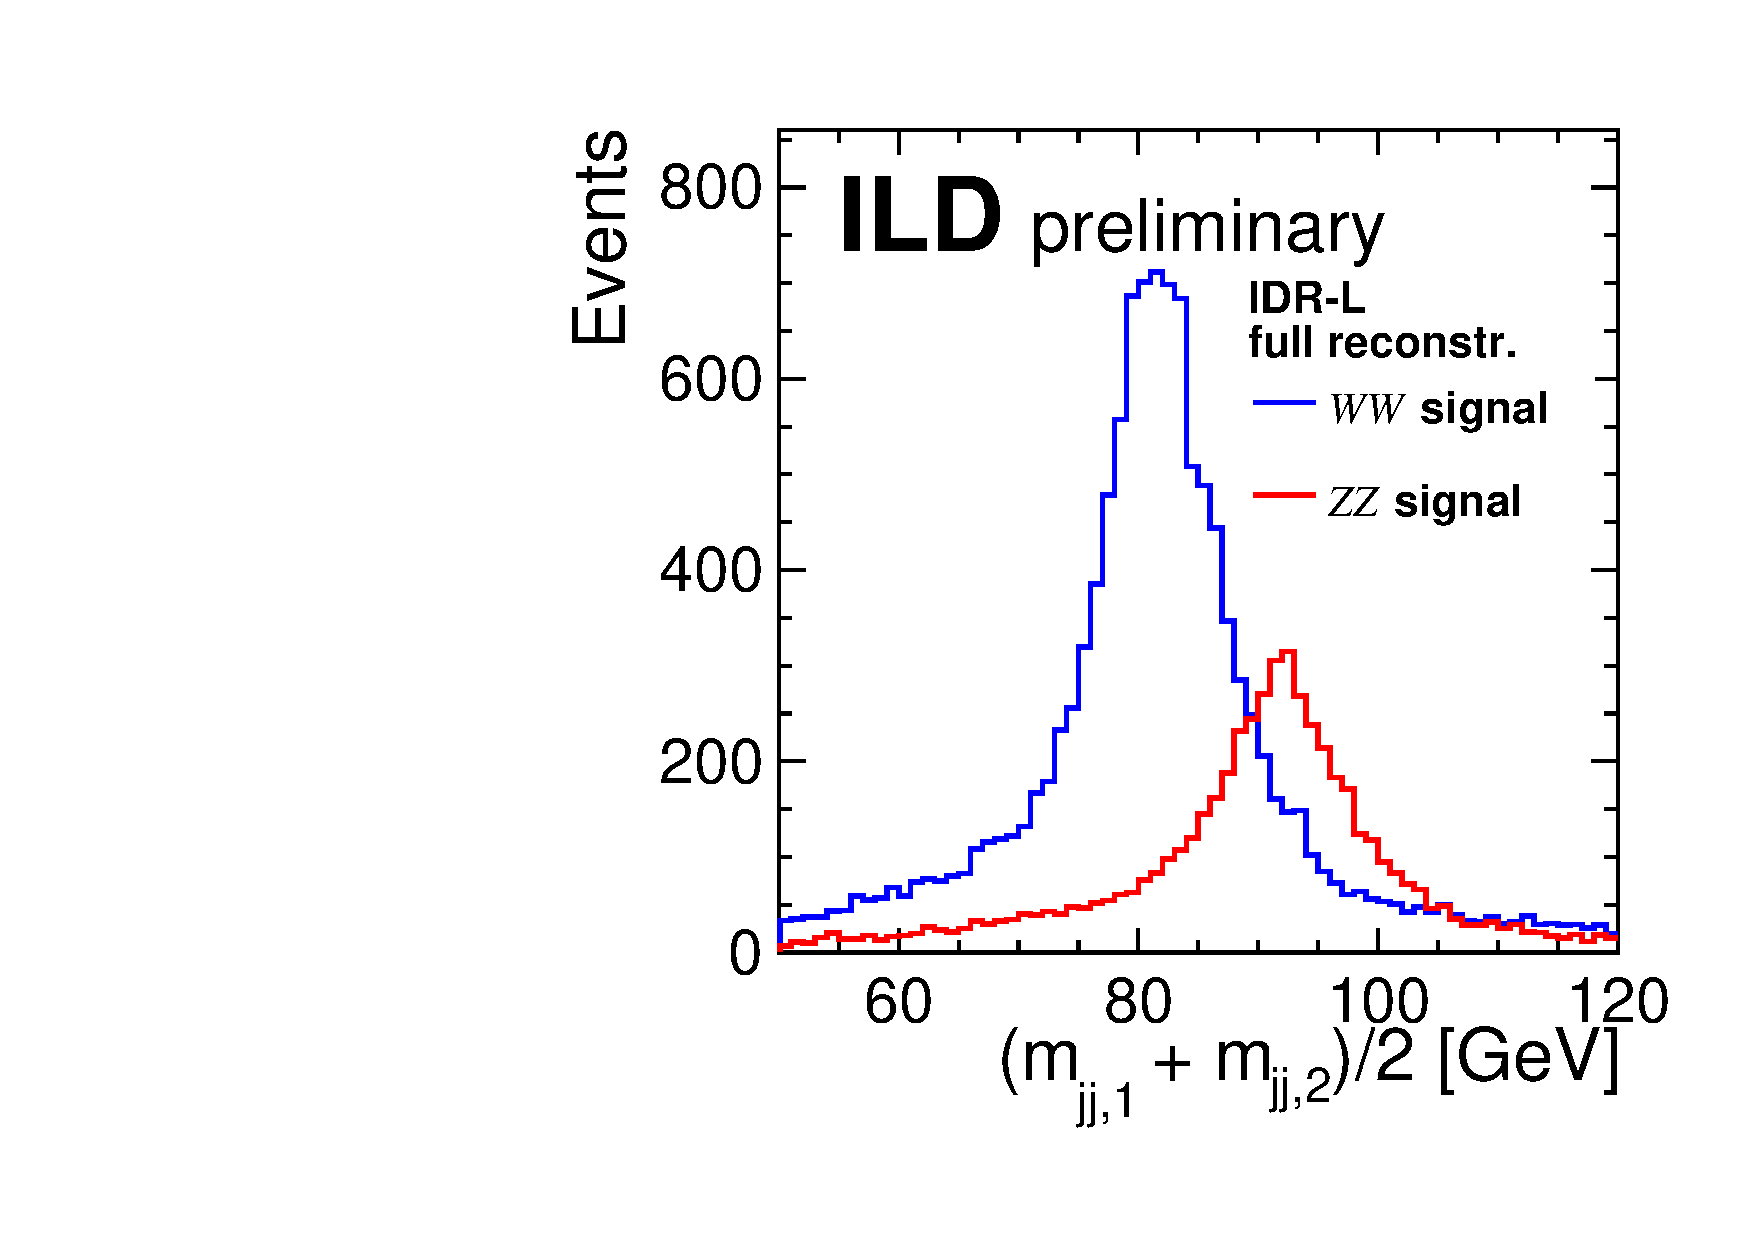
\includegraphics[width=\textwidth]{\imagepath/MassPlots/l5_m}
    \caption{}
    \label{SUBFIG:IDRL_m}
  \end{subfigure}%
  \begin{subfigure}[t]{0.5\textwidth}
    \centering
    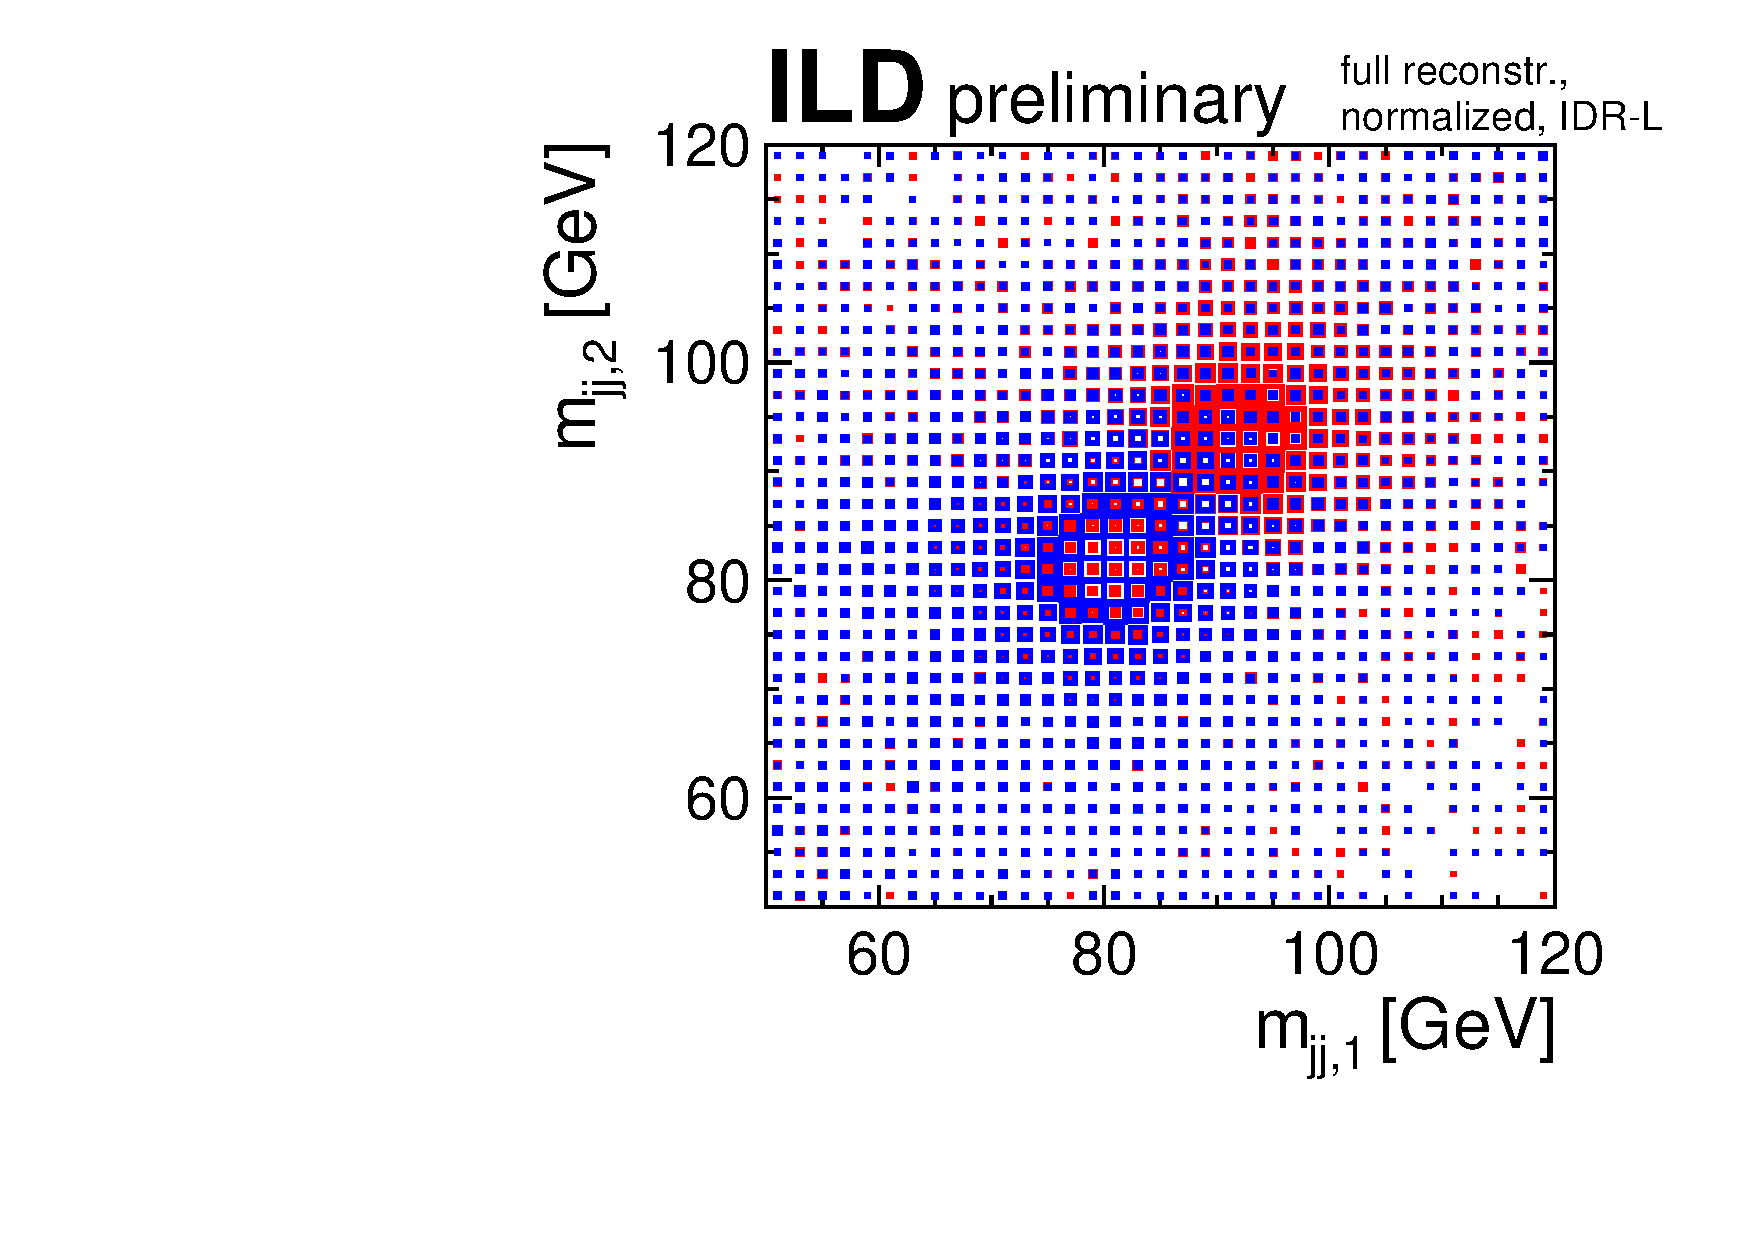
\includegraphics[width=\textwidth]{\imagepath/MassPlots/m_m_rec}
    \caption{}
    \label{SUBFIG:IDRL_m_m}
  \end{subfigure}
  \caption{
    Cool plots.
    \subfigref{SUBFIG:IDRL_m} This one is nice. 
    \subfigref{SUBFIG:IDRL_m_m} But this one is also nice.
  }
  \label{FIG:MassPlotsIDRL}
\end{figure}

In contrast, tables can sometimes be a bit dense and should be used with caution (see tab.~\ref{TAB:WWZZSeparationEfficiencies}).

\begin{table}
  \centering
  \caption{
    A table that shows numbers.
  } 
  \label{TAB:WWZZSeparationEfficiencies}
  \begin{tabular}{|l|l|l|l|l|} \hline
    Level & \multicolumn{4}{c|}{$\epsilon_{WW/ZZ} [\%]$} \\ \cline{2-5}
     & \multicolumn{2}{c|}{full $m_{VV}$ range} & \multicolumn{2}{c|}{$m_{VV}>500\,$GeV} \\ \cline{2-5}
     & IDR-L & IDR-S & IDR-L & IDR-S \\ \hline \hline
    Full reconstruction  & 71.1 & 71.5 & 73.0 & 72.9 \\ \hline
    Cheated overlay & 79.6 & 79.4 & 84.6 & 84.0 \\ \hline
    Cheated jets & 86.3 & 85.9 & 86.2 & 85.6 \\ \hline
    Cheated bosons & 88.4 & 88.1 & 86.6 & 86.1 \\ \hline
    No semi-leptonic events & 94.4 & 94.3 & 92.6 & 92.5 \\ \hline
  \end{tabular}
\end{table}

It is trivial that equations are important in physics so one could write one like this

\begin{equation} \label{EQ:ExactNeutrinoSolution}
  p_{\nu,\parallel} = \frac{1}{2 \cdot D} \cdot \left(-A \, \pm\, \sqrt{A^2 - BD} \right) \, 
\end{equation}

and describe all its symbols.

And one can even write many aligned ones

 \begin{align}
  A & =p_{\text{vis},\parallel} \cdot ( 2 p_{\text{vis},\perp}^2 + m_{\text{vis}}^2 - m_{X}^2) \\
  B & =4 p_{\text{vis},\perp}^2 \cdot E_{\text{vis}}^2 - ( 2 p_{\text{vis},\perp}^2 + m_{\text{vis}}^2 - m_{X}^2 )^2 \\
  D & =E_{\text{vis}}^2- p_{\text{vis},\parallel}^2
\end{align}

and also remember to describe all symbols used!

Sometimes it can be helpful for long formulas and $\eP\eM$ collisions to define shortcuts (see end of \texttt{Preamble.tex}).

If Feynman-diagrams are necessary (they are) then one can even do that (see fig.~\ref{FEY:SignalProcess}).

\begin{figure} 
  \centering
  \begin{tikzpicture}
  \begin{feynman}[scale=1] % using the vertex in brackets () allows fixing of vertex
    \vertex[blob] (m) at (0, 0) {\contour{white}{}};
    \vertex (a) at (-1,-1);
    \vertex (b) at ( 1.25,-1) ;
    \vertex (c) at (-1, 1);
    \vertex (d) at ( 1.25, 1) ;
    \vertex (q1) at ( 3,-1.5) {$q$};
    \vertex (q2) at ( 3,-0.5) {$\bar{q}$};
    \vertex (q3) at ( 3, 1.5) {$q$};
    \vertex (q4) at ( 3, 0.5) {$\bar{q}$};
    \vertex (i1) at (-2.5,-1) {$e^-$};
    \vertex (o1) at ( 2.5,-2.25) {$\nu_e$};
    \vertex (i2) at (-2.5, 1) {$e^+$};
    \vertex (o2) at ( 2.5, 2.25) {$\bar{\nu_e}$};
    \diagram* {
      (i1) -- [fermion] (a) -- [fermion] (o1) ,
      (i2) -- [anti fermion] (c) -- [anti fermion] (o2) ,
      (a) -- [photon, edge label=$W^-$] (m),
      (m) -- [photon, edge label=$W^+$] (c),
      (b) -- [photon, edge label=$W^-/Z$, swap] (m),
      (d) -- [photon, edge label=$W^+/Z$] (m),
      (b) -- [fermion] (q1),
      (b) -- [anti fermion] (q2),
      (d) -- [fermion] (q3),
      (d) -- [anti fermion] (q4),
    };
  \end{feynman}
\end{tikzpicture}
  \caption{Pseudo Feynman diagram of vector boson scattering in the $\nu\nubar q\qbar q\qbar$ final state at $\eP\eM$ colliders.}
  \label{FEY:SignalProcess}
\end{figure}